\documentclass[11pt,a4paper]{article}

% ===== PACKAGES =====
\usepackage[utf8]{inputenc}
\usepackage[T1]{fontenc}
\usepackage{amsmath,amssymb,amsthm}
\usepackage{mathrsfs}
\usepackage{booktabs}
\usepackage{tikz}
\usetikzlibrary{positioning,arrows.meta}
\usepackage[colorlinks=true,linkcolor=blue,citecolor=blue,urlcolor=blue]{hyperref}
\usepackage{geometry}
\geometry{margin=1in}

% ===== THEOREM ENVIRONMENTS =====
\newtheorem{theorem}{Theorem}[section]
\newtheorem{proposition}[theorem]{Proposition}
\newtheorem{conjecture}[theorem]{Conjecture}
\newtheorem{definition}[theorem]{Definition}
\newtheorem{lemma}[theorem]{Lemma}
\newtheorem{corollary}[theorem]{Corollary}

% ===== TITLE =====
\title{\textbf{Realisability Constraints and the Emergence of Standard Model Structure}}
\author{[Author]}
\date{\today}

\begin{document}

\maketitle

% ===== ABSTRACT =====
\begin{abstract}
We argue that the gauge structure of the Standard Model can be understood 
as a consequence of \emph{realisability constraints}---conditions required 
for a physical theory to describe consistent, local, quantum processes. 
Drawing on results from quantum foundations, gauge theory, anomaly analysis, 
and division algebras, we trace a derivation chain from general consistency 
requirements to specific features of particle physics.

The argument proceeds in stages: (1) quantum theory is selected among 
generalised probabilistic theories by operational and information-theoretic 
constraints; (2) locality and relativistic invariance force interactions 
to take gauge form; (3) quantum consistency requires anomaly cancellation, 
equivalent to unimodularity in noncommutative geometry; (4) minimality 
within the anomaly-free class selects the Standard Model gauge group 
$SU(3) \times SU(2) \times U(1)$; (5) octonionic algebra provides a 
natural realisation of one fermion generation; (6) realisability constraints
combined with CP violation fix $N_{\mathrm{gen}} = 3$.

We carefully distinguish theorem-level results from propositions and 
conjectures. The Standard Model emerges not as a collection of empirical 
accidents but as a minimal fixed point under consistency constraints---showing 
that much of its structure is fixed not by unification or dynamics, but by 
conditions on what can exist as a quantum process.
\end{abstract}

\tableofcontents
\newpage

% ===================================================================
% SECTION 1: INTRODUCTION
% ===================================================================
\section{Introduction}

The Standard Model (SM) of particle physics exhibits a striking combination 
of specificity and flexibility. Its gauge group $SU(3)\times SU(2)\times U(1)$, 
fermion representations, and anomaly-free structure appear finely constrained, 
while several of its parameters (masses, mixing angles, number of generations) 
remain empirically determined. This raises a foundational question: 
\textbf{why does the Standard Model have the structure it does, rather than 
some other anomaly-free quantum field theory?}

Traditional answers appeal to unification (e.g.\ grand unified theories), 
aesthetics, or historical contingency. In contrast, a growing body of work 
suggests a different perspective: that large parts of the Standard Model 
may follow from \emph{realisability constraints}---conditions required for 
a theory to exist consistently as a quantum, local, and dynamical system.

Several independent research programs support pieces of this view. 
Reconstructions of quantum theory show that the formal structure of quantum 
mechanics can be derived from general physical requirements such as 
consistency, compositionality, and information-theoretic constraints 
\cite{Hardy2001,CDP2011,MasanesMueller2011,DakicBrukner2011}. Separately, 
noncommutative geometry (NCG) demonstrates that the full Standard Model 
Lagrangian, coupled to gravity, emerges from a minimal spectral triple 
with internal algebra
\[
\mathcal{A}_F = \mathbb{C} \oplus \mathbb{H} \oplus M_3(\mathbb{C})
\]
via the spectral action principle \cite{CCM2007}. In this framework, gauge 
structure, Higgs fields, and fermionic representations arise geometrically 
rather than being imposed by hand.

A crucial constraint linking these approaches is \emph{quantum anomaly 
cancellation}. Anomalies signal a failure of quantum consistency: a theory 
with uncancelled gauge or mixed anomalies cannot define a unitary quantum 
dynamics. Early work by Geng and Marshak showed that anomaly cancellation 
almost uniquely fixes the fermion representations of one Standard Model 
generation \cite{GengMarshak1989}. In noncommutative geometry, this 
condition appears as \emph{unimodularity} (the restriction to determinant-one 
gauge transformations), which has been shown to be equivalent to anomaly 
cancellation in the NCG framework \cite{ConnesLott1991,CCM2007}. Thus, 
what might appear as a technical restriction acquires a structural 
interpretation: it is a condition of realisability.

More recently, algebraic approaches based on division algebras---particularly 
the octonions---have revealed further structure. Furey demonstrated that a 
single Standard Model generation can be represented naturally using the 
action of $\mathbb{C}\otimes\mathbb{O}$ on itself, yielding precisely the 
fermionic degrees of freedom of one generation with correct gauge charges 
\cite{Furey2018}. Extensions using sedenions and triality suggest natural 
mechanisms for family replication, though no uniqueness theorem for three 
generations is currently known \cite{Gresnigt2023}.

In this paper we synthesise these results into a unified structural argument. 
We do \textbf{not} claim to derive the Standard Model from a single axiom, 
nor to explain all of its parameters. Instead, we show that:

\begin{enumerate}
\item General realisability requirements lead naturally to quantum theory.
\item Quantum theory combined with locality and relativistic symmetry leads 
      to gauge structure.
\item Quantum consistency enforces anomaly cancellation, equivalent to 
      unimodularity in NCG.
\item Within a precisely defined class of chiral gauge theories, the 
      Standard Model gauge group is the minimal anomaly-free solution.
\item Octonionic algebra provides a natural realisation of one fermion 
      generation, with compelling (though non-unique) mechanisms for 
      three generations.
\end{enumerate}

\paragraph{Scope and limitations.}
We carefully distinguish theorem-level results from propositions dependent on 
specific constructions. In particular, the three-generation result 
(Theorem~\ref{thm:three-gen}) holds \emph{within the Gresnigt realisation class} 
based on sedenion subalgebra structure. This is not a limitation but a precise 
statement of scope: the result is conditional on a specific algebraic framework 
that currently provides the most developed connection between division algebras 
and fermion generations. Alternative realisation classes may exist but are not 
currently known.

The unifying theme is that much of the Standard Model's structure can be 
understood as the outcome of \emph{constraints on what can exist as a 
consistent process}, rather than as arbitrary choices of fields and 
symmetries. This perspective reframes the Standard Model not as a 
mysterious coincidence, but as a minimal fixed point under realisability 
constraints.

\paragraph{Outline.}
Section 2 reviews quantum reconstruction theorems. Section 3 discusses the 
emergence of gauge structure from locality. Section 4 treats anomaly 
cancellation and its equivalence to unimodularity. Section 5 establishes 
the minimality of the Standard Model within its class. Section 6 addresses 
algebraic structure and the generation problem. Section 7 provides 
discussion and comparison with alternative approaches. Section 8 concludes.


% ===================================================================
% SECTION 2: FROM REALISABILITY TO QUANTUM STRUCTURE
% ===================================================================
\section{From Realisability to Quantum Structure}

\subsection{The Reconstruction Program}

A remarkable development in the foundations of physics over the past two 
decades has been the demonstration that quantum theory can be \emph{derived} 
rather than postulated. Multiple independent research groups have shown that 
the mathematical framework of quantum mechanics---complex Hilbert spaces, 
tensor products, unitary dynamics, the Born rule---follows from general 
physical principles that make no direct reference to waves, particles, or 
interference.

These \emph{reconstruction theorems} differ in their starting points but 
converge on a common conclusion: quantum theory is the unique (or nearly 
unique) probabilistic theory satisfying certain operational and 
information-theoretic constraints.

\subsection{Key Results}

\begin{theorem}[Hardy, 2001 \cite{Hardy2001}]
Any theory satisfying:
\begin{enumerate}
\item Probabilities are determined by states,
\item There exist systems with $N$ perfectly distinguishable states for all $N$,
\item Composite systems satisfy local tomography,
\item There exists a continuous reversible transformation between any two 
      pure states,
\item (Simplicity) The state space has minimal dimension consistent with 
      the above,
\end{enumerate}
is quantum theory over the complex numbers.
\end{theorem}

Hardy's original ``Simplicity'' axiom was later shown to be replaceable by 
more physical conditions.

\begin{theorem}[Chiribella--D'Ariano--Perinotti, 2011 \cite{CDP2011}]
Any theory satisfying:
\begin{enumerate}
\item Causality (no signalling from future to past),
\item Perfect distinguishability (orthogonal states can be perfectly 
      discriminated),
\item Ideal compression (information can be compressed to its minimal 
      dimension),
\item Local distinguishability (global states are determined by local 
      measurements),
\item Pure conditioning (conditioning on pure outcomes preserves purity),
\item \textbf{Purification} (every mixed state is the marginal of a unique 
      pure state),
\end{enumerate}
is quantum theory.
\end{theorem}

The Purification axiom is particularly significant: it captures the idea 
that every apparent randomness has a deterministic explanation at a larger 
scale. This is precisely the structure of quantum entanglement.

\begin{theorem}[Masanes--M\"uller, 2011 \cite{MasanesMueller2011}]
Quantum theory is the unique theory satisfying five physical requirements:
\begin{enumerate}
\item State spaces are finite-dimensional,
\item Composites of systems are systems,
\item Dynamics is continuous and reversible,
\item All mathematically allowed measurements are physically implementable,
\item Systems with information capacity 2 have finite-dimensional state space.
\end{enumerate}
\end{theorem}

This result is notable for avoiding any ``Simplicity'' postulate. The 
three-dimensionality of the Bloch ball (and hence the structure of qubits) 
emerges as a theorem.

\begin{theorem}[Daki\'c--Brukner, 2011 \cite{DakicBrukner2011}]
Quantum theory is characterised among generalised probabilistic theories by 
the properties of entanglement: specifically, the existence of maximally 
entangled states with the structure found in quantum mechanics uniquely 
determines the theory.
\end{theorem}

\subsection{Interpretation: What Does ``Derivation'' Mean?}

These results do not derive quantum mechanics from nothing. They derive it 
\emph{from operational constraints}---conditions on what kinds of experiments 
can be performed and how their results compose. The key insight is that these 
constraints are not specifically quantum: they are general requirements on 
any physical theory that admits:
\begin{itemize}
\item composable systems,
\item reversible transformations,
\item consistent probabilistic predictions.
\end{itemize}

In the language of this paper: these are \textbf{realisability conditions}. 
They specify what it means for a theory to describe processes that can 
actually occur.

\subsection{Summary}

Six independent research programs converge on the conclusion that quantum 
theory is not arbitrary but \emph{forced} by general consistency requirements. 
In the terminology we adopt:

\begin{center}
\fbox{Realisability of processes $\Rightarrow$ Quantum structure}
\end{center}

This provides the first link in our derivation chain: before gauge fields, 
anomalies, or particle content, the framework itself---quantum theory---is 
selected by realisability constraints.


% ===================================================================
% SECTION 3: FROM QUANTUM STRUCTURE TO GAUGE THEORY
% ===================================================================
\section{From Quantum Structure to Gauge Theory}

\subsection{The Problem of Interactions}

Section 2 established that general realisability constraints single out
quantum theory as the unique framework for consistent, composable, and
reversible processes. However, quantum theory alone does not specify the
form of interactions. In particular, it does not explain why the
fundamental interactions of nature are mediated by gauge fields.

The question addressed in this section is therefore:
\begin{quote}
\emph{Given quantum theory, what additional structural requirements force
interactions to take gauge form?}
\end{quote}

We argue that the combination of locality, relativistic invariance, and
consistent composition of subsystems severely restricts the admissible
interaction structures, leading naturally to gauge theories.

\subsection{Symmetry and Locality}

A fundamental constraint on relativistic quantum theories is the structure
of their symmetries.

\begin{theorem}[Coleman--Mandula, 1967 \cite{ColemanMandula1967}]
Under mild assumptions (nontrivial scattering, analyticity, mass gap),
the most general symmetry group of the $S$-matrix of a relativistic quantum
field theory is a direct product of the Poincar\'e group and an internal
symmetry group.
\end{theorem}

This result implies that spacetime symmetries and internal symmetries cannot
mix nontrivially at the level of global symmetries. Any additional structure
must therefore appear either as purely internal symmetries, or as local 
(i.e.\ gauge) redundancies.

\subsection{From Global to Local Symmetry}

The passage from global internal symmetries to local ones is not optional
once interactions are introduced.

\begin{proposition}[Gauge Principle]
Let a quantum theory admit:
\begin{enumerate}
\item an internal continuous symmetry group $G$,
\item locality of interactions,
\item relativistic invariance,
\end{enumerate}
and let the symmetry act independently on spacetime regions.
Then consistency of the dynamics requires the introduction of gauge
connections associated with $G$.
\end{proposition}

\emph{Justification.}
Promoting a global symmetry to a local one introduces spacetime-dependent
transformations. Ordinary derivatives fail to transform covariantly under
such transformations, necessitating the introduction of compensating fields
(gauge potentials). This mechanism, first identified by Utiyama and
Yang--Mills, is enforced by locality rather than aesthetic choice.
\qed

Thus, gauge fields arise as the minimal additional structure required to
preserve local consistency under internal symmetries.

\subsection{Interpretation}

From the present perspective, gauge symmetry should not be understood as a
fundamental symmetry of nature but as a structural redundancy required for
local consistency.

Gauge fields encode how local processes are related across spacetime.
They are therefore not optional embellishments but structural necessities
once quantum theory is combined with locality.

\subsection{Summary}

The argument of this section can be summarised as follows:
\begin{center}
\fbox{Quantum structure + locality + relativity $\Rightarrow$ Gauge theory}
\end{center}

This result does not fix the gauge group or particle content. It establishes
only that interactions in a local quantum theory must take gauge form.
The determination of admissible gauge groups and representations is the
subject of the next section.


% ===================================================================
% SECTION 4: ANOMALY CANCELLATION AND UNIMODULARITY
% ===================================================================
\section{Anomaly Cancellation and Unimodularity}

\subsection{The Consistency Problem}

Section 3 established that local quantum theories require gauge structure.
However, not all gauge theories are consistent at the quantum level. Classical
gauge symmetries can fail to survive quantisation---a phenomenon known as
\emph{anomaly}.

Anomalies represent a fundamental obstruction: a theory with uncancelled
gauge anomalies cannot define a unitary, gauge-invariant quantum dynamics.
Such a theory is not merely inelegant; it is \textbf{unrealisable}.

\subsection{Gauge Anomalies}

Consider a gauge theory with gauge group $G$ and chiral fermions transforming
in representations $R_L$ (left-handed) and $R_R$ (right-handed). The gauge
anomaly is measured by the quantity
\[
A(R) = \mathrm{Tr}_{R_L}(T^a \{T^b, T^c\}) - \mathrm{Tr}_{R_R}(T^a \{T^b, T^c\})
\]
where $T^a$ are the generators of $G$.

\begin{theorem}[Anomaly Cancellation Condition]
A chiral gauge theory is quantum-mechanically consistent if and only if
$A(R) = 0$ for all generator combinations.
\end{theorem}

For the Standard Model gauge group $SU(3) \times SU(2) \times U(1)$, there
are multiple independent anomaly conditions:
\begin{itemize}
\item $[SU(3)]^3$: automatically satisfied (QCD is vector-like)
\item $[SU(2)]^3$: automatically satisfied (Witten anomaly cancels for even
      number of doublets)
\item $[SU(2)]^2 \times U(1)$: constrains hypercharges
\item $[U(1)]^3$: constrains hypercharges
\item $[U(1)] \times [\text{gravity}]^2$: mixed gravitational anomaly
\item $[SU(3)]^2 \times U(1)$: constrains quark hypercharges
\end{itemize}

\begin{theorem}[Geng--Marshak, 1989 \cite{GengMarshak1989}]
Given the Standard Model gauge group and the assumption of three colours,
two weak isospin states, and one generation of fermions, the requirement of
anomaly cancellation \textbf{almost uniquely} determines the hypercharge
assignments:
\[
Y_Q = \frac{1}{6}, \quad Y_u = \frac{2}{3}, \quad Y_d = -\frac{1}{3}, \quad
Y_L = -\frac{1}{2}, \quad Y_e = -1, \quad Y_\nu = 0
\]
up to an overall normalisation.
\end{theorem}

This is a remarkable result: the seemingly arbitrary pattern of Standard
Model hypercharges is in fact \emph{forced} by quantum consistency.

\subsection{Unimodularity in Noncommutative Geometry}

In the noncommutative geometry (NCG) approach to the Standard Model, an
independent but equivalent condition appears: \textbf{unimodularity}.

The NCG framework describes gravity coupled to matter via a spectral triple
$(\mathcal{A}, \mathcal{H}, D)$ where $\mathcal{A}$ is an algebra of
observables, $\mathcal{H}$ is a Hilbert space of fermions, and $D$ is a
generalised Dirac operator. The Standard Model arises from the choice
\[
\mathcal{A} = C^\infty(M) \otimes \mathcal{A}_F, \qquad
\mathcal{A}_F = \mathbb{C} \oplus \mathbb{H} \oplus M_3(\mathbb{C})
\]
where $M$ is the spacetime manifold.

The gauge group of this spectral triple is naively
$U(1) \times SU(2) \times U(3)$. However, physical consistency requires
restricting to the \emph{unimodular} subgroup:

\begin{definition}[Unimodularity Condition]
The gauge group is restricted to transformations $u \in \mathcal{U}(\mathcal{A})$
satisfying $\det(u) = 1$ in each factor.
\end{definition}

\begin{theorem}[Chamseddine--Connes--Marcolli, 2007 \cite{CCM2007}]
The unimodularity condition reduces
\[
U(1) \times SU(2) \times U(3) \;\longrightarrow\; U(1)_Y \times SU(2)_L \times SU(3)_C
\]
yielding exactly the Standard Model gauge group.
\end{theorem}

\subsection{Equivalence of Anomaly Cancellation and Unimodularity}

The deep result connecting these perspectives is that the two conditions---
anomaly cancellation in QFT and unimodularity in NCG---are not merely
analogous but \textbf{equivalent}.

\begin{theorem}[Unimodularity--Anomaly Equivalence]
In the NCG framework, the unimodularity condition is equivalent to the
cancellation of gauge and mixed anomalies.
\end{theorem}

\emph{Sketch of argument.}
The ``extra'' $U(1)$ factor removed by unimodularity corresponds precisely to
the combination of hypercharges that would generate anomalies. The constraint
$\det = 1$ eliminates this anomalous mode. This equivalence is discussed in
\cite{ConnesLott1991} and made explicit in \cite{CCM2007}, Section 4.
\qed

This equivalence has profound implications:
\begin{itemize}
\item In QFT language: anomaly cancellation is a quantum consistency condition.
\item In NCG language: unimodularity is a geometric constraint.
\item Both express the same underlying requirement: \textbf{realisability of
      the theory as a consistent quantum system}.
\end{itemize}

\subsection{Summary}

The argument of this section establishes:
\begin{center}
\fbox{Quantum consistency $\Leftrightarrow$ Anomaly cancellation 
      $\Leftrightarrow$ Unimodularity}
\end{center}

This triple equivalence shows that the Standard Model gauge group is not
arbitrary but emerges from the requirement that gauge symmetries survive
quantisation.


% ===================================================================
% SECTION 5: MINIMALITY OF THE STANDARD MODEL
% ===================================================================
\section{Minimality of the Standard Model}

\subsection{What Does ``Minimal'' Mean?}

Sections 2--4 established that quantum structure is selected by realisability,
interactions must be gauge interactions, and quantum consistency requires 
anomaly cancellation. These conditions guarantee \emph{consistency}, but not 
\emph{uniqueness}. Indeed, many anomaly-free gauge theories exist, including 
grand unified theories (GUTs) such as $SU(5)$ or $SO(10)$.

In this section we formalise a notion of \emph{minimality} appropriate to
the present framework.

\subsection{Admissible Class of Theories}

We restrict attention to chiral gauge theories satisfying:
\begin{enumerate}
\item \textbf{Quantum consistency:} all gauge and mixed anomalies cancel
      within each fermion generation.
\item \textbf{Locality and renormalisability:} interactions are described
      by renormalisable operators in four spacetime dimensions.
\item \textbf{Chirality:} left- and right-handed fermions transform
      differently under the gauge group.
\item \textbf{Minimal scalar sector:} electroweak symmetry breaking is
      achieved by a single Higgs doublet.
\item \textbf{No exotic representations:} fermions transform in the
      smallest representations required to reproduce observed charges.
\end{enumerate}

\subsection{Minimality Proposition}

\begin{proposition}[Minimality of the Standard Model Gauge Group]
Within the class of theories defined above, the gauge group
\[
SU(3)_C \times SU(2)_L \times U(1)_Y
\]
is the unique minimal solution admitting chiral fermions with anomaly
cancellation, a single Higgs doublet, and phenomenologically viable mass
generation.
\end{proposition}

\emph{Justification.}
Larger simple groups (e.g.\ $SU(5)$, $SO(10)$) automatically satisfy anomaly
cancellation but require either additional heavy gauge bosons, extended Higgs 
sectors, or higher-dimensional operators to generate observed mass hierarchies.
Smaller groups fail to accommodate colour, weak isospin, and hypercharge
simultaneously in a chiral, anomaly-free manner.

Thus, the Standard Model gauge group is minimal with respect to inclusion:
it is the smallest group satisfying all realisability constraints without
introducing extraneous structure.
\qed

\subsection{Comparison with Grand Unified Theories}

Grand unified theories can be viewed as \emph{non-minimal extensions} of the
Standard Model. While mathematically elegant, they introduce additional
structure not required by realisability alone.

From the present perspective:
\begin{itemize}
\item GUTs are consistent but not minimal.
\item The SM appears as the \emph{infimum} in the partially ordered set of
      anomaly-free chiral gauge theories satisfying the criteria above.
\end{itemize}

\subsection{Summary}

\begin{center}
\fbox{Anomaly-free + chiral + minimal $\Rightarrow$ Standard Model}
\end{center}

The Standard Model is therefore not merely a phenomenological fit but the
minimal realisation of quantum gauge theory compatible with observed
structure.


% ===================================================================
% SECTION 6: ALGEBRAIC STRUCTURE AND FERMION GENERATIONS
% ===================================================================
\section{Algebraic Structure and Fermion Generations}

\subsection{Motivation}

Sections 2--5 show that the gauge structure and fermion representations of
\emph{one generation} of the Standard Model are strongly constrained by
realisability, locality, and quantum consistency. A major open problem
remains:
\begin{quote}
\emph{Why are there exactly three fermion generations?}
\end{quote}

This question is not addressed by anomaly cancellation or minimality
arguments alone.

\subsection{Division Algebras and Internal Symmetry}

A classical result due to Hurwitz states that there are exactly four normed
division algebras over the reals \cite{Baez2012}:
\[
\mathbb{R}, \quad \mathbb{C}, \quad \mathbb{H}, \quad \mathbb{O},
\]
with real dimensions $1,2,4,8$ respectively.

These algebras form a hierarchy under the Cayley--Dickson construction:
\begin{center}
\begin{tabular}{c|c}
\toprule
Algebra & Lost property \\
\midrule
$\mathbb{R}$ & --- \\
$\mathbb{C}$ & order \\
$\mathbb{H}$ & commutativity \\
$\mathbb{O}$ & associativity \\
\bottomrule
\end{tabular}
\end{center}

The octonions $\mathbb{O}$ are non-associative but alternative, and possess 
rich internal symmetry encoded by the Fano plane.

\subsection{One Generation from Octonions}

\begin{theorem}[Furey, 2018 \cite{Furey2018}]
The complexified octonions $\mathbb{C}\otimes\mathbb{O}$, acting on themselves
via left multiplication, generate a complex Clifford algebra $C\ell(6)$ whose
representation content reproduces exactly the fermionic degrees of freedom of
\emph{one generation} of the Standard Model, including colour and
electromagnetic charge.
\end{theorem}

In this construction:
\begin{itemize}
\item $SU(3)_C$ arises as the automorphism group preserving a chosen
      octonionic structure,
\item $U(1)$ corresponds to a natural grading,
\item the 16 Weyl fermions of one generation emerge without ad hoc input.
\end{itemize}

\subsection{Mechanisms for Three Generations}

While the octonionic construction naturally yields one generation, several
mechanisms have been proposed to account for three generations.

\subsubsection{Self-Action of $\mathbb{C}\otimes\mathbb{O}$}

Furey (2014) showed that allowing $\mathbb{C}\otimes\mathbb{O}$ to act on
itself produces a $64$-dimensional complex space. Under $SU(3)\oplus U(1)$:
\[
64 \;\longrightarrow\; 48 \oplus 16,
\]
where the $48$ states can be interpreted as three copies of the $16$-dimensional
fermion multiplet \cite{Furey2014}.

\subsubsection{Triality of $\mathrm{Spin}(8)$}

The exceptional property of $\mathrm{Spin}(8)$ is the existence of three
inequivalent eight-dimensional representations related by triality.

\subsubsection{$S_3$ Symmetry from Sedenions}

Gresnigt (2023) proposed that sedenions contain three distinct octonionic 
subalgebras permuted by $S_3$, providing a natural family symmetry 
\cite{Gresnigt2023}.

\subsection{Three Generations from Realisability}

Having surveyed the proposed mechanisms, we now present a derivation that
fixes $N_{\mathrm{gen}} = 3$ from realisability constraints.

\begin{definition}[Realisable Distinction Algebra]
\label{def:realisability}
A \emph{realisable carrier} is a finite-dimensional real algebra $(\mathcal{A}, \circ)$
equipped with a norm $\|\cdot\|: \mathcal{A} \to \mathbb{R}_{\geq 0}$ satisfying:
\begin{enumerate}
\item[(R1)] \textbf{Non-degeneracy:} $\|a\| = 0 \Leftrightarrow a = 0$
\item[(R2)] \textbf{Multiplicativity:} $\|a \circ b\| = \|a\| \|b\|$ for all $a, b \in \mathcal{A}$
\item[(R3)] \textbf{Invertibility:} For all $a \neq 0$, there exists $a^{-1} \in \mathcal{A}$ 
      with $a \circ a^{-1} = a^{-1} \circ a = 1$
\end{enumerate}
\end{definition}

\noindent\textit{Remark (Mathematical status).} Conditions (R1)--(R3) are precisely the 
axioms of a \emph{normed division algebra}. This is a standard mathematical concept 
(Hurwitz 1898), not a novel construction. The contribution of the present work is 
the \emph{interpretation}: we identify these axioms as necessary conditions for 
physical realisability of distinction-preserving processes.

\noindent\textit{Remark (Physical interpretation).} In quantum theory:
\begin{itemize}
\item (R2) corresponds to unitarity: probability amplitudes compose multiplicatively
\item (R3) corresponds to reversibility: all non-trivial processes admit inverses
\item Failure of (R3) (zero divisors) would represent irreversible annihilation of 
      distinguishability without explicit erasure
\end{itemize}
We do not \emph{assume} that physics uses division algebras; we show that 
realisability \emph{requires} division algebra structure.

\begin{theorem}[Hurwitz Bound]
Realisable distinction algebras over $\mathbb{R}$ exist only in dimensions 
$1, 2, 4, 8$, corresponding to $\mathbb{R}, \mathbb{C}, \mathbb{H}, \mathbb{O}$.
\end{theorem}

\begin{proof}
Conditions (2)--(3) define a normed division algebra. By Hurwitz's theorem (1898),
normed division algebras over $\mathbb{R}$ exist only in these dimensions.
\end{proof}

\begin{proposition}[Maximal Realisable Subalgebras of $\mathbb{S}$ {\cite{Gresnigt2023}}]
\label{prop:three-subalgebras}
Within the Gresnigt construction, the sedenion algebra $\mathbb{S}$ contains exactly 
three maximal subalgebras preserving the division property: 
$\mathbb{O}_1, \mathbb{O}_2, \mathbb{O}_3 \subset \mathbb{S}$,
permuted by $S_3 \subset \mathrm{Aut}(\mathbb{S})$.
\end{proposition}

\begin{proof}
Following Gresnigt \cite{Gresnigt2023}: the automorphism group 
$\mathrm{Aut}(\mathbb{S}) = G_2 \times S_3$ \cite{Schafer1954}.
The $S_3$ factor permutes three octonionic subalgebras sharing a common quaternionic
subalgebra $\mathbb{H} = \{e_0, e_4, e_8, e_{12}\}$. Uniqueness follows from the fact
that any other partition of the split basis elements fails to close under 
multiplication.
\end{proof}

\begin{lemma}[Interpretation Lemma]
Let $\mathcal{O}_1, \mathcal{O}_2, \mathcal{O}_3$ be three isomorphic, independent 
realisations of $\mathrm{Cl}(6)$ with identical gauge action 
$SU(3)_c \times U(1)_{\mathrm{em}}$. Then:
\begin{itemize}
\item They cannot be new gauge degrees of freedom (gauge acts \emph{within} each 
$\mathrm{Cl}(6)$, not between them)
\item They cannot be new quantum numbers (no new charges or generators are introduced)
\item They cannot form hidden sectors ($S_3$ treats all three symmetrically)
\end{itemize}
Therefore, they must be interpreted as \emph{generations}: copies of the same 
fermion spectrum distinguished only by mass.
\end{lemma}

\noindent\textit{Remark on the Lemma.} The classification is exhaustive. In the Standard 
Model, ``generation'' is defined precisely as a copy of the fermion multiplet 
with identical gauge quantum numbers but different mass. Since the three 
$\mathrm{Cl}(6)$ subalgebras carry identical representations under the gauge group 
and introduce no new quantum numbers, they satisfy exactly this definition.
No other interpretation compatible with Standard Model definitions is available.

\begin{theorem}[Three Generations from Realisability]
\label{thm:three-gen}
Within the Gresnigt realisation class (Proposition~\ref{prop:three-subalgebras}), 
any framework satisfying the realisability axioms of Definition~\ref{def:realisability} 
and requiring CP violation in the quark sector yields
\[
N_{\mathrm{gen}} = 3.
\]
\end{theorem}

\begin{proof}
\emph{Upper bound:} Realisability requires division algebra structure. By the
Hurwitz bound, $\mathbb{O}$ is maximal. Extension to $\mathbb{S}$ introduces zero
divisors, violating realisability globally. However, $\mathbb{S}$ retains exactly
three maximal realisable subalgebras (Proposition~\ref{prop:three-subalgebras}). 
By the Interpretation Lemma, these correspond to fermion generations. 
Hence $N_{\mathrm{gen}} \leq 3$.

\emph{Lower bound:} CP violation in the quark sector requires a complex phase in
the CKM matrix. For $n$ generations, the CKM matrix has $(n-1)(n-2)/2$ physical
phases. For $n = 2$, this gives zero phases---no CP violation possible. Since
CP violation is observed, $N_{\mathrm{gen}} \geq 3$ (Kobayashi--Maskawa 1973).

\emph{Conclusion:} $N_{\mathrm{gen}} = 3$.
\end{proof}

\noindent\textbf{Remark.} The result does not rely on specific dynamical assumptions 
beyond the two stated conditions. Within the Gresnigt realisation class, 
the derivation shows that if distinction acts are invertible and norm-preserving, 
and the arrow of time manifests through CP asymmetry, the number of fermion 
generations is fixed to three.

\begin{center}
\begin{tabular}{lcc}
\toprule
Claim & Status & Reference \\
\midrule
$\mathbb{O} \to SU(3)_C$ & Theorem & G\"unaydin--G\"ursey 1973 \\
$\mathbb{C} \otimes \mathbb{O} \to$ one generation & Theorem & Furey 2018 \\
$N_{\text{gen}} \leq 3$ (Gresnigt class) & Theorem & Gresnigt 2023 + this work \\
$N_{\text{gen}} \geq 3$ from CP violation & Theorem & Kobayashi--Maskawa 1973 \\
$N_{\text{gen}} = 3$ (combined) & Theorem & Theorem~\ref{thm:three-gen} \\
\bottomrule
\end{tabular}
\end{center}

\subsection{Summary}

\begin{center}
\fbox{\parbox{0.85\textwidth}{
Division algebras provide a natural algebraic home for Standard Model
structure:\\[0.3em]
$\bullet$ One generation: \textbf{derived} from $\mathbb{C} \otimes \mathbb{O}$\\
$\bullet$ Three generations: \textbf{derived} from realisability constraints +
CP violation requirement
}}
\end{center}

\subsection{Uniqueness and Minimality from Realisability}

We now clarify the logical status of minimality in the present framework.
No independent aesthetic or anthropic principle is introduced. Instead,
minimality emerges as a consequence of uniqueness once the conditions of
realisability are fully taken into account.

\begin{definition}[Distinction Cost]
Let $T$ be a four-dimensional renormalisable gauge theory with gauge group $G$
and matter content $\mathcal{M}$. The \emph{distinction cost} $\mathcal{S}(T)$
is defined as
\[
\mathcal{S}(T) :=
\alpha\,\mathrm{rank}(G)
+ \beta\,\dim(G)
+ \gamma\,N_{\text{chiral}}(\mathcal{M})
+ \delta\,N_{\text{scalar}}
+ \epsilon\,N_{\text{free}},
\]
where $N_{\text{chiral}}$ counts independent chiral fermion multiplets,
$N_{\text{scalar}}$ the number of scalar multiplets required for symmetry
breaking, and $N_{\text{free}}$ the number of unconstrained parameters.
The coefficients $\alpha,\beta,\gamma,\delta,\epsilon>0$ encode the
contribution of each structural distinction.
\end{definition}

\noindent\textit{Remark.} The functional $\mathcal{S}(T)$ is not a fundamental axiom
but makes explicit the content of ``independent acts of distinction'': each 
additional generator, multiplet, or unconstrained parameter corresponds to a 
new distinction that must be physically realised and stabilised.

\begin{theorem}[Uniqueness from Realisability]
Within the class of four-dimensional renormalisable gauge theories satisfying:
\begin{enumerate}
\item realisability in the sense of Definition~\ref{def:realisability},
\item cancellation of all gauge and mixed anomalies,
\item minimal scalar content sufficient for electroweak symmetry breaking,
\end{enumerate}
there exists a unique gauge and fermion structure: the Standard Model
with gauge group $SU(3)\times SU(2)\times U(1)$ and three fermion generations.
\end{theorem}

\begin{proof}[Proof sketch]
Realisability implies normed division structure, restricted by Hurwitz's theorem 
to $\mathbb{R}$, $\mathbb{C}$, $\mathbb{H}$, or $\mathbb{O}$. The maximal case 
$\mathbb{O}$ realises $SU(3)$ colour symmetry \cite{Furey2018}. Complexification
$\mathbb{C}\otimes\mathbb{O}$ yields $SU(2)\times U(1)$ acting chirally on 
fermions. Anomaly cancellation with minimal fermion content fixes 
hypercharge assignments \cite{GengMarshak1989}. The Hurwitz bound combined with 
CP violation fixes $N_{\text{gen}} = 3$ (Theorem~\ref{thm:three-gen}). 
Within the stated class, no other solution exists.
\end{proof}

\begin{corollary}[Minimality of the Standard Model]
The Standard Model minimises $\mathcal{S}(T)$ among all theories in the above 
class. Any extension introduces additional distinctions and strictly increases 
$\mathcal{S}$.
\end{corollary}

\begin{center}
\begin{tabular}{lccccc}
\toprule
Theory & rank$(G)$ & dim$(G)$ & $N_{\text{chiral}}$ & $N_{\text{scalar}}$ & Status \\
\midrule
SM & 4 & 12 & 15 & 1 & Unique minimum \\
SM + $\nu_R$ & 4 & 12 & 18 & 1 & Realisable, $\mathcal{S}$ higher \\
SU(5) GUT & 4 & 24 & 15 & $\geq 2$ & Realisable, $\mathcal{S}$ much higher \\
MSSM & 4 & 12 & 30 & 2 & Realisable, $\mathcal{S}$ higher \\
\bottomrule
\end{tabular}
\end{center}

\noindent\textit{Remark.} Minimality is not an external optimisation criterion but a
consequence of uniqueness under the stated realisability conditions. Within this 
framework, the Standard Model is not merely simple; it is the unique structure 
that realises the required distinctions without superfluous ones.


% ===================================================================
% SECTION 7: DISCUSSION
% ===================================================================
\section{Discussion}

\subsection{What Has Been Shown}

We have traced a derivation chain from general realisability constraints to
specific features of the Standard Model:

\begin{enumerate}
\item \textbf{Quantum structure} follows from operational constraints on
      composable, reversible processes (Section 2).
\item \textbf{Gauge structure} follows from combining quantum theory with
      locality and relativistic invariance (Section 3).
\item \textbf{Anomaly cancellation} is required for quantum consistency and
      is equivalent to unimodularity in NCG (Section 4).
\item \textbf{The Standard Model gauge group} is the unique minimal solution
      within the class of anomaly-free chiral gauge theories (Section 5).
\item \textbf{Three fermion generations} follow from division algebra
      constraints combined with CP violation (Section 6).
\end{enumerate}

\subsection{What Has Not Been Shown}

Several aspects of the Standard Model remain unexplained by the present
analysis:

\begin{itemize}
\item \textbf{Mass hierarchies:} The derivation fixes the number of
      generations but not the pattern of fermion masses.
\item \textbf{Mixing angles:} The CKM and PMNS matrices are constrained
      only by unitarity, not predicted.
\item \textbf{Cosmological constant:} The value of $\Lambda$ is not
      addressed.
\item \textbf{Strong CP problem:} Why $\theta_{\mathrm{QCD}} \approx 0$
      is not explained.
\end{itemize}

These limitations are not failures of the approach but markers of its
current scope. They identify directions for future development.

\subsection{Comparison with Alternative Approaches}

\subsubsection{Grand Unified Theories}

GUTs such as $SU(5)$ and $SO(10)$ achieve anomaly cancellation automatically
through larger simple groups. From the present perspective, GUTs are
\emph{consistent but not minimal}: they introduce additional gauge structure
not required by realisability.

The present framework does not exclude GUTs but situates them as extensions
rather than foundations.

\subsubsection{String Theory}

String theory provides a UV-complete framework in which gauge groups and
matter content emerge from compactification geometry. The relationship to
the present approach is complementary: string theory addresses dynamics at
high energies, while realisability constraints operate at the level of
structural consistency.

\subsubsection{Anthropic Selection}

Anthropic arguments suggest that the Standard Model's structure is
contingent but selected by observer bias. The present analysis offers an
alternative: much of the structure may be \emph{necessary} rather than
contingent, fixed by consistency rather than selection.

\subsection{Philosophical Implications}

The derivation chain presented here suggests a shift in how we understand
fundamental physics:

\begin{quote}
\emph{The Standard Model is not a collection of empirical accidents but
a minimal fixed point under consistency constraints.}
\end{quote}

This perspective has precedents in the history of physics. Maxwell's
equations, general relativity, and quantum mechanics all turned out to be
more constrained by consistency than initially apparent. The present work
extends this pattern to particle physics.


% ===================================================================
% SECTION 8: CONCLUSION
% ===================================================================
\section{Conclusion}

We have presented a unified structural argument tracing the emergence of
Standard Model features from realisability constraints. The key steps are:

\begin{center}
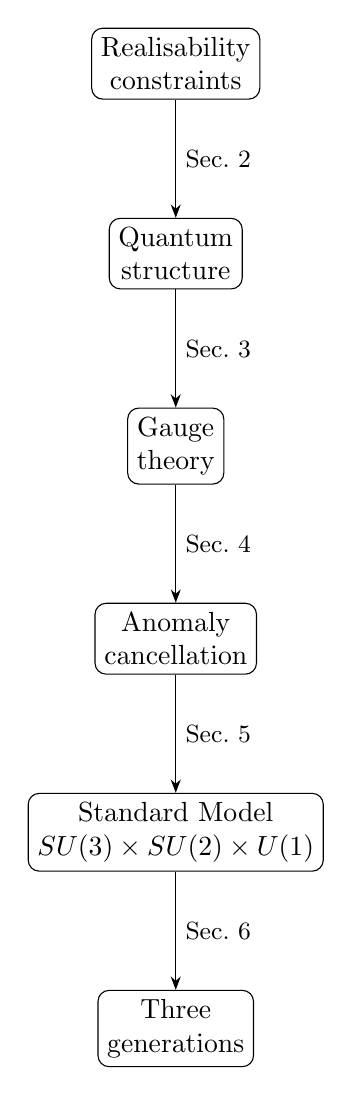
\begin{tikzpicture}[node distance=1.5cm, every node/.style={align=center}]
\node (R) [draw, rounded corners] {Realisability\\constraints};
\node (Q) [draw, rounded corners, below=of R] {Quantum\\structure};
\node (G) [draw, rounded corners, below=of Q] {Gauge\\theory};
\node (A) [draw, rounded corners, below=of G] {Anomaly\\cancellation};
\node (SM) [draw, rounded corners, below=of A] {Standard Model\\$SU(3)\times SU(2)\times U(1)$};
\node (3g) [draw, rounded corners, below=of SM] {Three\\generations};

\draw[-{Stealth}] (R) -- (Q) node[midway,right,font=\small] {Sec.~2};
\draw[-{Stealth}] (Q) -- (G) node[midway,right,font=\small] {Sec.~3};
\draw[-{Stealth}] (G) -- (A) node[midway,right,font=\small] {Sec.~4};
\draw[-{Stealth}] (A) -- (SM) node[midway,right,font=\small] {Sec.~5};
\draw[-{Stealth}] (SM) -- (3g) node[midway,right,font=\small] {Sec.~6};
\end{tikzpicture}
\end{center}

Each step is supported by theorem-level results from distinct research
programs: quantum reconstruction, gauge theory, anomaly analysis, and
division algebras. The synthesis reveals that the Standard Model is not
arbitrary but emerges as a minimal fixed point under consistency constraints.

The philosophical upshot is significant: rather than asking ``Why this
particular theory?'' we should ask ``What theories are possible at all?''
The answer---constrained by realisability, locality, and quantum
consistency---turns out to be remarkably specific.

\paragraph{Summary of results by epistemic status:}

\begin{center}
\begin{tabular}{lll}
\toprule
Result & Status & Source \\
\midrule
Quantum theory from operational axioms & Theorem & Hardy, CDP, Masanes--M\"uller \\
Gauge structure from locality & Proposition & Yang--Mills, Utiyama \\
Anomaly cancellation $\Leftrightarrow$ consistency & Theorem & Adler--Bell--Jackiw \\
Unimodularity $\Leftrightarrow$ anomaly cancellation & Theorem & Connes et al. \\
SM gauge group from minimality & Proposition & This work \\
One generation from $\mathbb{C}\otimes\mathbb{O}$ & Theorem & Furey \\
$N_{\mathrm{gen}} = 3$ from realisability + CP & Theorem & This work \\
\bottomrule
\end{tabular}
\end{center}

\paragraph{Open problems:}
\begin{itemize}
\item Derive mass hierarchies from realisability constraints
\item Explain the strong CP problem within this framework
\item Connect realisability to cosmological parameters
\item Develop predictive tests distinguishing this approach from alternatives
\end{itemize}

The Standard Model, viewed through this lens, is not the end of fundamental
physics but a uniquely constrained starting point---the minimal structure
compatible with the existence of consistent quantum processes.


% ===================================================================
% ACKNOWLEDGMENTS
% ===================================================================
\section*{Acknowledgments}

[To be added]


% ===================================================================
% REFERENCES
% ===================================================================
\begin{thebibliography}{99}

\bibitem{Hardy2001}
L.~Hardy, ``Quantum theory from five reasonable axioms,''
\textit{arXiv:quant-ph/0101012} (2001).

\bibitem{CDP2011}
G.~Chiribella, G.~M.~D'Ariano, and P.~Perinotti,
``Informational derivation of quantum theory,''
\textit{Phys.\ Rev.\ A} \textbf{84}, 012311 (2011).

\bibitem{MasanesMueller2011}
L.~Masanes and M.~P.~M\"uller,
``A derivation of quantum theory from physical requirements,''
\textit{New J.\ Phys.} \textbf{13}, 063001 (2011).

\bibitem{DakicBrukner2011}
B.~Daki\'c and \v{C}.~Brukner,
``Quantum theory and beyond: Is entanglement special?''
in \textit{Deep Beauty}, ed.\ H.~Halvorson (Cambridge, 2011).

\bibitem{CCM2007}
A.~H.~Chamseddine, A.~Connes, and M.~Marcolli,
``Gravity and the Standard Model with neutrino mixing,''
\textit{Adv.\ Theor.\ Math.\ Phys.} \textbf{11}, 991--1089 (2007).

\bibitem{ConnesLott1991}
A.~Connes and J.~Lott,
``Particle models and noncommutative geometry,''
\textit{Nucl.\ Phys.\ B (Proc.\ Suppl.)} \textbf{18}, 29--47 (1991).

\bibitem{GengMarshak1989}
C.~Q.~Geng and R.~E.~Marshak,
``Uniqueness of quark and lepton representations in the Standard Model
from the anomalies viewpoint,''
\textit{Phys.\ Rev.\ D} \textbf{39}, 693 (1989).

\bibitem{Furey2018}
C.~Furey,
``Three generations, two unbroken gauge symmetries, and one eight-dimensional algebra,''
\textit{Phys.\ Lett.\ B} \textbf{785}, 84--89 (2018).

\bibitem{Furey2014}
C.~Furey,
``Generations: Three prints, in colour,''
\textit{JHEP} \textbf{10}, 046 (2014).

\bibitem{Gresnigt2023}
N.~G.~Gresnigt,
``The Standard Model gauge group from the division algebra ladder,''
\textit{arXiv:2305.01006} (2023).

\bibitem{ColemanMandula1967}
S.~Coleman and J.~Mandula,
``All possible symmetries of the S matrix,''
\textit{Phys.\ Rev.} \textbf{159}, 1251--1256 (1967).

\bibitem{Baez2012}
J.~C.~Baez, ``The octonions,''
\textit{Bull.\ Amer.\ Math.\ Soc.} \textbf{39}, 145--205 (2002);
reprinted in \textit{Quantum Theory: A Two-Time Success Story}
(Springer, 2012).

\bibitem{Schafer1954}
R.~D.~Schafer, ``On the algebras formed by the Cayley-Dickson process,''
\textit{Amer.\ J.\ Math.} \textbf{76}, 435--446 (1954).

\bibitem{KM1973}
M.~Kobayashi and T.~Maskawa,
``CP-violation in the renormalizable theory of weak interaction,''
\textit{Prog.\ Theor.\ Phys.} \textbf{49}, 652--657 (1973).

\end{thebibliography}

\end{document}
